\section{Pipeline Architecture [Rahat Rafiq]}\label{sec:architecture_sec}

\begin{figure}[h]
    \centering
    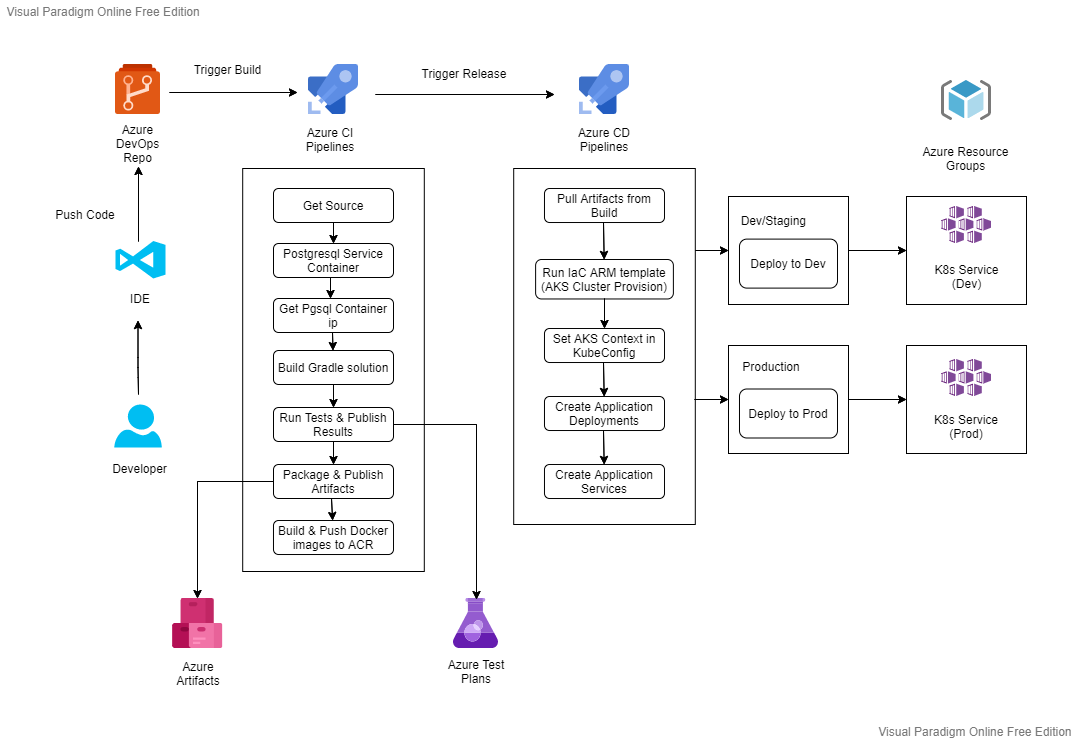
\includegraphics[width=15cm]{images/Rahat/Azure CI-CD Pipline Architecture.png}
    \caption{Azure DevOps CI-CD Architecture}
    \label{fig:azure-devops-ci-cd-pipeline-architecture}
\end{figure}

Application source code is developed and extended when necessary in local environment of developers and then pushed to the Azure DevOps Repos for version controlling. Azure Repos will serve as the primary source code-base for building, testing and deploying the spring boot application in azure CI-CD pipeline. Both continuous integration and continuous deployment pipeline is configured in the same service of azure devops "Azure Pipelines". Whenever a developer pushes a new commit to the specific branch of azure repos where a trigger is configured a subsequent build in the CI pipeline will start executing. CI pipeline first pulls the source code from azure repos, then it builds the application, performs the specified tests and publish test results in the "Azure Test Plans" service. After that CI pipeline packages the generated artifacts from the build and drops it in the "azure artifacts" service, from where these artifacts are available to CD pipelines. In the last step CI pipeline builds the docker image of the dvdstore application by utilizing a dockerfile available in the azure repo branch and pushes it to the specified azure container registry in azure portal. CD pipeline triggers are configured at inbound events at specific azure container registries. Thus CD pipeline triggers a new release whenever CI pipeline pushes an docker image to specified container registries. First it fetches the generated artifacts of the corresponding CI build from azure artifacts directory. Then Infrastructure as Code (IaC) tool "Azure Resource Manager" or ARM is integrated with the CD pipeline job that dynamically provisions an azure kubernetes service (AKS) cluster with appropriate load balancing architecture and deploys it to the targeted deployment environment in the azure portal with the help of a service connection. Finally CD pipeline creates kubernetes deployment objects for dvdstore application and postgresql database back-end and it also exposes the dvdstore deployment to a external ip address or FQDN that extends the IaC implemented load-balancing architecture. Finally the application is accessible from the resource dashboard of the AKS cluster, which conveniently lists the FQDN or public ip of externally accessible services and ingresses of that cluster. ~\ref{fig:azure-devops-ci-cd-pipeline-architecture} 
